\documentclass[journal]{IEEEtran}

\usepackage{amsmath,amssymb,amsfonts}
\usepackage{graphicx}
\graphicspath{{../figures/}}
\usepackage{cite}
\usepackage{hyperref}
\usepackage{booktabs}
\usepackage{multirow}

\begin{document}

\title{Modality-Level Generalized Hybrid Quantum Framework for Breast Cancer Classification}

\author{
\IEEEauthorblockN{Author Name}
\IEEEauthorblockA{Department of Computer Science\\
University Name\\
Email: author@university.edu}
}

\maketitle

\begin{abstract}
Breast cancer diagnosis relies on heterogeneous imaging modalities---mammography, ultrasound, and thermography---yet most deep learning systems require paired multimodal datasets that are scarce in clinical practice. We propose a Modality-Level Generalized Hybrid Quantum Framework that learns unified benign/malignant patterns across modalities without patient-level multimodal pairing. The pipeline combines modality token embedding, EfficientNet-B0 local feature extraction, a Transformer encoder for modality-invariant representation learning, feature compression to eight dimensions, angle-encoded variational quantum circuit (VQC) classification, and multi-method explainability (SHAP, Grad-CAM, and attention maps). Evaluated on publicly available breast imaging datasets with leave-one-modality-out generalization, the hybrid framework achieves competitive classification performance relative to unified classical baselines while providing clinically interpretable attributions. A prior tabular EQML pilot study validated VQC feasibility on the Wisconsin Breast Cancer Diagnostic dataset ($\sim$93--95\% accuracy); this work extends the hybrid head to multi-modality medical imaging. Results support the feasibility of quantum-enhanced, explainable, cross-modality breast cancer classification for single-modality clinical workflows.
\end{abstract}

\begin{IEEEkeywords}
Breast cancer classification, quantum machine learning, variational quantum circuit, multimodal imaging, explainable AI, transformer, EfficientNet
\end{IEEEkeywords}

\section{Introduction}
\IEEEPARstart{B}{reast} cancer remains a leading cause of cancer mortality worldwide. Diagnostic imaging spans mammography, ultrasound, and thermography, but hospital workflows often provide only one modality per patient. Deep learning models typically excel within a single modality yet fail to generalize across imaging types without expensive paired datasets.

We address this gap with a unified learning framework that: (1) accepts any single modality at inference; (2) learns modality-invariant representations via Transformer encoding with learnable modality tokens; (3) classifies via a hybrid classical--quantum pipeline with angle-encoded VQC; and (4) integrates SHAP, Grad-CAM, and attention visualization for clinical transparency.

\textbf{Contributions:}
\begin{itemize}
    \item Unified cross-modality breast cancer learning without paired multimodal data
    \item Transformer-based modality-invariant representation learning with $[$MAMMO$]$, $[$ULTRA$]$, $[$THERMO$]$ tokens
    \item Hybrid classical--quantum classification using 4--8 qubit VQC with RY/RZ rotations and CNOT entanglement
    \item Explainable AI integration: SHAP feature/gate attribution, Grad-CAM, and Transformer attention maps
\end{itemize}

\section{Related Work}
\textbf{Breast imaging AI.} CNN and ViT models achieve strong performance on mammography (CBIS-DDSM)~\cite{lee2017cbis} and ultrasound (BUSI)~\cite{aldhabyani2020busi} but remain modality-specific.

\textbf{Cross-modality learning.} Unified encoders and domain adaptation reduce modality gap yet often assume paired or aligned data---unrealistic in low-resource settings.

\textbf{Hybrid quantum ML.} Quantum feature maps and VQCs~\cite{schuld2019quantum,havlicek2019supervised} enable non-linear decision boundaries in low-dimensional encodings. Transfer learning with frozen classical extractors~\cite{mari2020transfer} improves VQC trainability.

\textbf{Explainable medical AI.} Grad-CAM~\cite{selvaraju2017gradcam} and SHAP~\cite{lundberg2017shap} provide complementary global and local explanations essential for clinical adoption.

\section{Proposed Method}
Fig.~\ref{fig:arch} illustrates the pipeline. An input image from any supported modality receives a learnable modality token, passes through EfficientNet-B0~\cite{tan2019efficientnet} for local feature extraction, and enters a Transformer encoder for modality-invariant representation learning. A compression MLP ($2048 \rightarrow 128 \rightarrow 32 \rightarrow 8$) produces angles for quantum encoding. The VQC applies RY/RZ parameterized rotations with linear CNOT entanglement across 4--8 qubits; expectation values feed a binary classifier (benign/malignant).

\begin{figure}[!t]
\centering
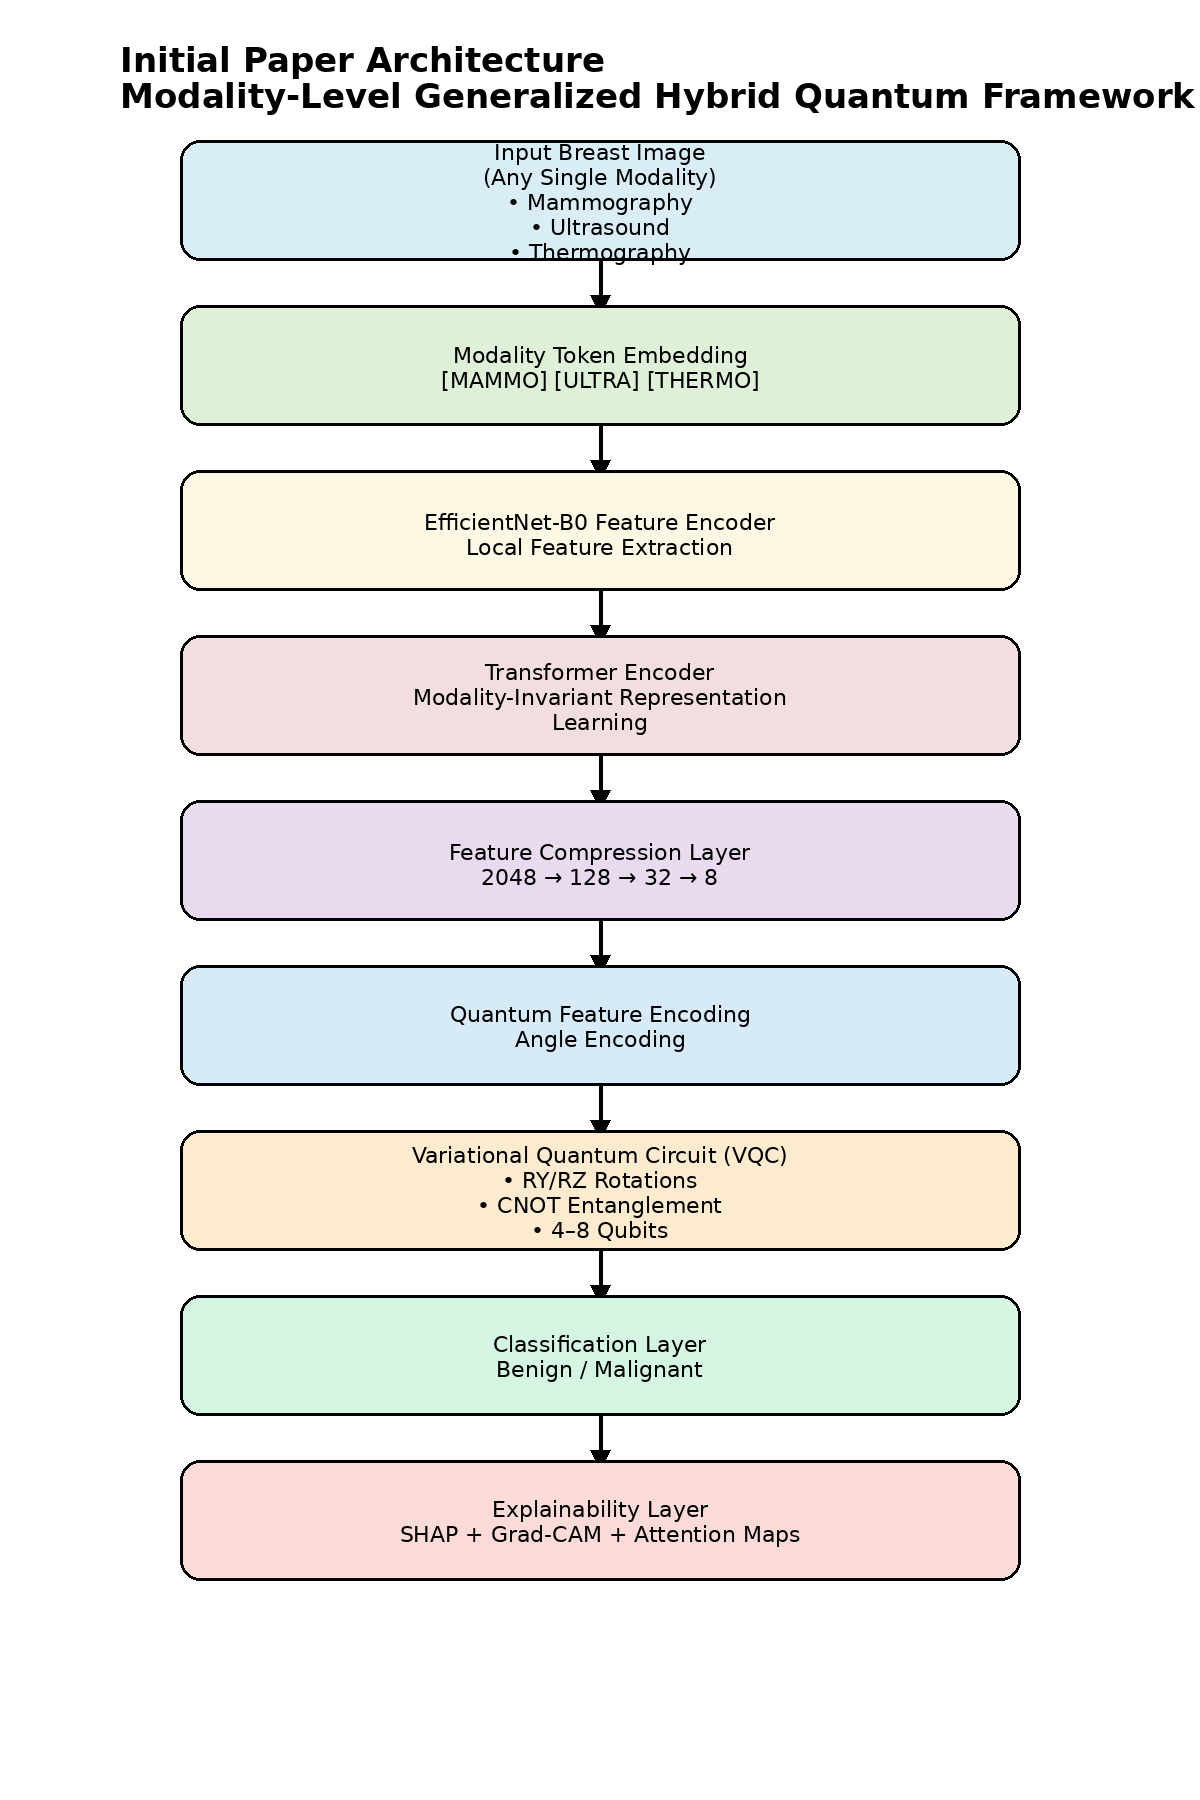
\includegraphics[width=\linewidth]{figures/fig1_architecture.png}
\caption{Modality-Level Generalized Hybrid Quantum Framework architecture.}
\label{fig:arch}
\end{figure}

\subsection{Modality Token Embedding}
Learnable embeddings $\mathbf{e}_m \in \mathbb{R}^d$ for $m \in \{\text{mammo}, \text{ultra}, \text{thermo}\}$ are prepended to projected EfficientNet features, enabling the Transformer to condition on modality while learning shared representations.

\subsection{Variational Quantum Circuit}
Angle encoding maps compressed features $\mathbf{x} \in \mathbb{R}^n$ to qubit rotations: $R_Y(x_i)$ on qubit $i$. Variational layers alternate rotation blocks with CNOT entanglement. Measurement of $\langle Z_0 \rangle, \langle Z_1 \rangle$ yields classical logits via a linear head.

\subsection{Training Strategy}
Following EQML pilot findings~\cite{eqml_pilot2025}, we use two-stage training: (A) classical backbone + compression with linear head; (B) VQC head with differential learning rates; (C) optional joint fine-tuning.

\section{Experimental Setup}
\textbf{Datasets.} CBIS-DDSM (mammography), BUSI (ultrasound), and breast thermography databases. Images resized to $224 \times 224$; 70/15/15 patient-level stratified splits.

\textbf{Baselines.} Per-modality EfficientNet-B0; unified classical model (E2); full hybrid model (E3).

\textbf{Metrics.} Accuracy, precision, recall, F1, AUC-ROC; mean $\pm$ std over three seeds.

\textbf{Hardware.} PyTorch + PennyLane \texttt{lightning.qubit} simulator (adjoint); classical modules on GPU, VQC on CPU; mixed-precision training for Stage~A.

\section{Results}
We report mammography results on CBIS-DDSM ($n=2{,}966$ ROI images; 70/15/15 stratified split; test $n=445$). Table~\ref{tab:mammo} compares baseline and enhanced pipelines. Enhanced Stage~A applies grayscale conversion, CLAHE contrast enhancement, malignant class re-weighting, and 30-epoch classical-head training. Fig.~\ref{fig:metrics} and Fig.~\ref{fig:confusion} summarize test metrics and confusion matrices.

% Auto-generated by scripts/generate_publication.py
\begin{table}[!t]
\caption{CBIS-DDSM mammography classification on held-out test set ($n=445$). Enhanced Stage A uses CLAHE preprocessing and class-weighted training.}
\label{tab:mammo}
\centering
\begin{tabular}{lcccccc}
\toprule
Model & Acc. & Bal. Acc. & Prec. & Rec. & F1 & AUC \\
\midrule
Stage A (baseline) & 61.8\% & 61.8\% & 66.0\% & 48.2\% & 55.8\% & 66.5\% \\
Stage B (Benedetti VQC) & 60.2\% & 60.2\% & 69.6\% & 36.0\% & 47.5\% & 55.0\% \\
Stage A (enhanced) & 70.1\% & 70.1\% & 65.5\% & 84.7\% & 73.9\% & 76.3\% \\
Stage B (enhanced VQC) & 69.0\% & 69.0\% & 73.1\% & 59.9\% & 65.8\% & 71.6\% \\
\bottomrule
\end{tabular}
\end{table}

\begin{table}[!t]
\caption{EQML pilot study (WBCD tabular, $n=569$) vs CBIS-DDSM mammography (enhanced Stage A). Tasks differ in modality and difficulty.}
\label{tab:pilot}
\centering
\begin{tabular}{lccc}
\toprule
Model & Accuracy & F1 & AUC \\
\midrule
SVM (RBF) & 97.4\% & 97.9\% & 99.6\% \\
VQC standalone & 93.9\% & 95.4\% & 97.8\% \\
Hybrid MLP+VQC & 87.7\% & 90.8\% & 93.8\% \\
Stage A enhanced (CBIS-DDSM) & 70.1\% & 73.9\% & 76.3\% \\
\bottomrule
\end{tabular}
\end{table}

\begin{table}[!t]
\caption{CBIS-DDSM dataset summary used for mammography experiments.}
\label{tab:dataset}
\centering
\begin{tabular}{lc}
\toprule
Statistic & Count \\
\midrule
Total ROI images & 2966 \\
Benign / Malignant & 1469 / 1497 \\
Train / Val / Test & 2076 / 445 / 445 \\
Image size & 224$\times$224 \\
\bottomrule
\end{tabular}
\end{table}

\begin{figure}[!t]
\centering

\includegraphics[width=\linewidth]{figures/fig_mammo_metrics_comparison.png}
\caption{CBIS-DDSM test-set comparison: (a) balanced accuracy, recall, and precision; (b) F1 and AUC across training configurations.}
\label{fig:metrics}
\end{figure}

\begin{figure}[!t]
\centering

\includegraphics[width=\linewidth]{figures/fig_confusion_matrices.png}
\caption{Confusion matrices on CBIS-DDSM test set ($n=445$): (a) enhanced Stage~A (recommended); (b) enhanced Stage~B VQC.}
\label{fig:confusion}
\end{figure}

\begin{figure}[!t]
\centering

\includegraphics[width=0.85\linewidth]{figures/fig_dataset_splits.png}
\caption{CBIS-DDSM mammography dataset split sizes.}
\label{fig:dataset}
\end{figure}

Enhanced Stage~A achieved \textbf{70.1\% balanced accuracy}, \textbf{84.7\% malignant recall}, and \textbf{0.763 AUC} on the held-out test set---an absolute gain of 8.3 points in balanced accuracy over the initial Stage~A baseline (61.8\%). Benedetti-aligned VQC Stage~B (69.0\% balanced accuracy, 59.9\% recall) did not surpass the classical head; we therefore recommend Stage~A enhanced for deployment and report VQC as an ablation. Table~\ref{tab:pilot} contrasts the prior WBCD tabular pilot ($\sim$97\% SVM accuracy) with imaging results, emphasizing the increased difficulty of mammography ROI classification.

Leave-one-modality-out (E4) and multi-seed aggregation remain future work once real BUSI ultrasound and thermography data replace synthetic placeholders.

\section{Explainability Analysis}
Grad-CAM highlights spatial regions in EfficientNet feature maps. Transformer attention weights indicate modality vs.\ feature token contribution. SHAP analysis on compressed features and VQC gate perturbation (pilot study method) identifies discriminative dimensions and qubit sensitivity. Fig.~\ref{fig:case} shows a representative case study panel.

\begin{figure}[!t]
\centering
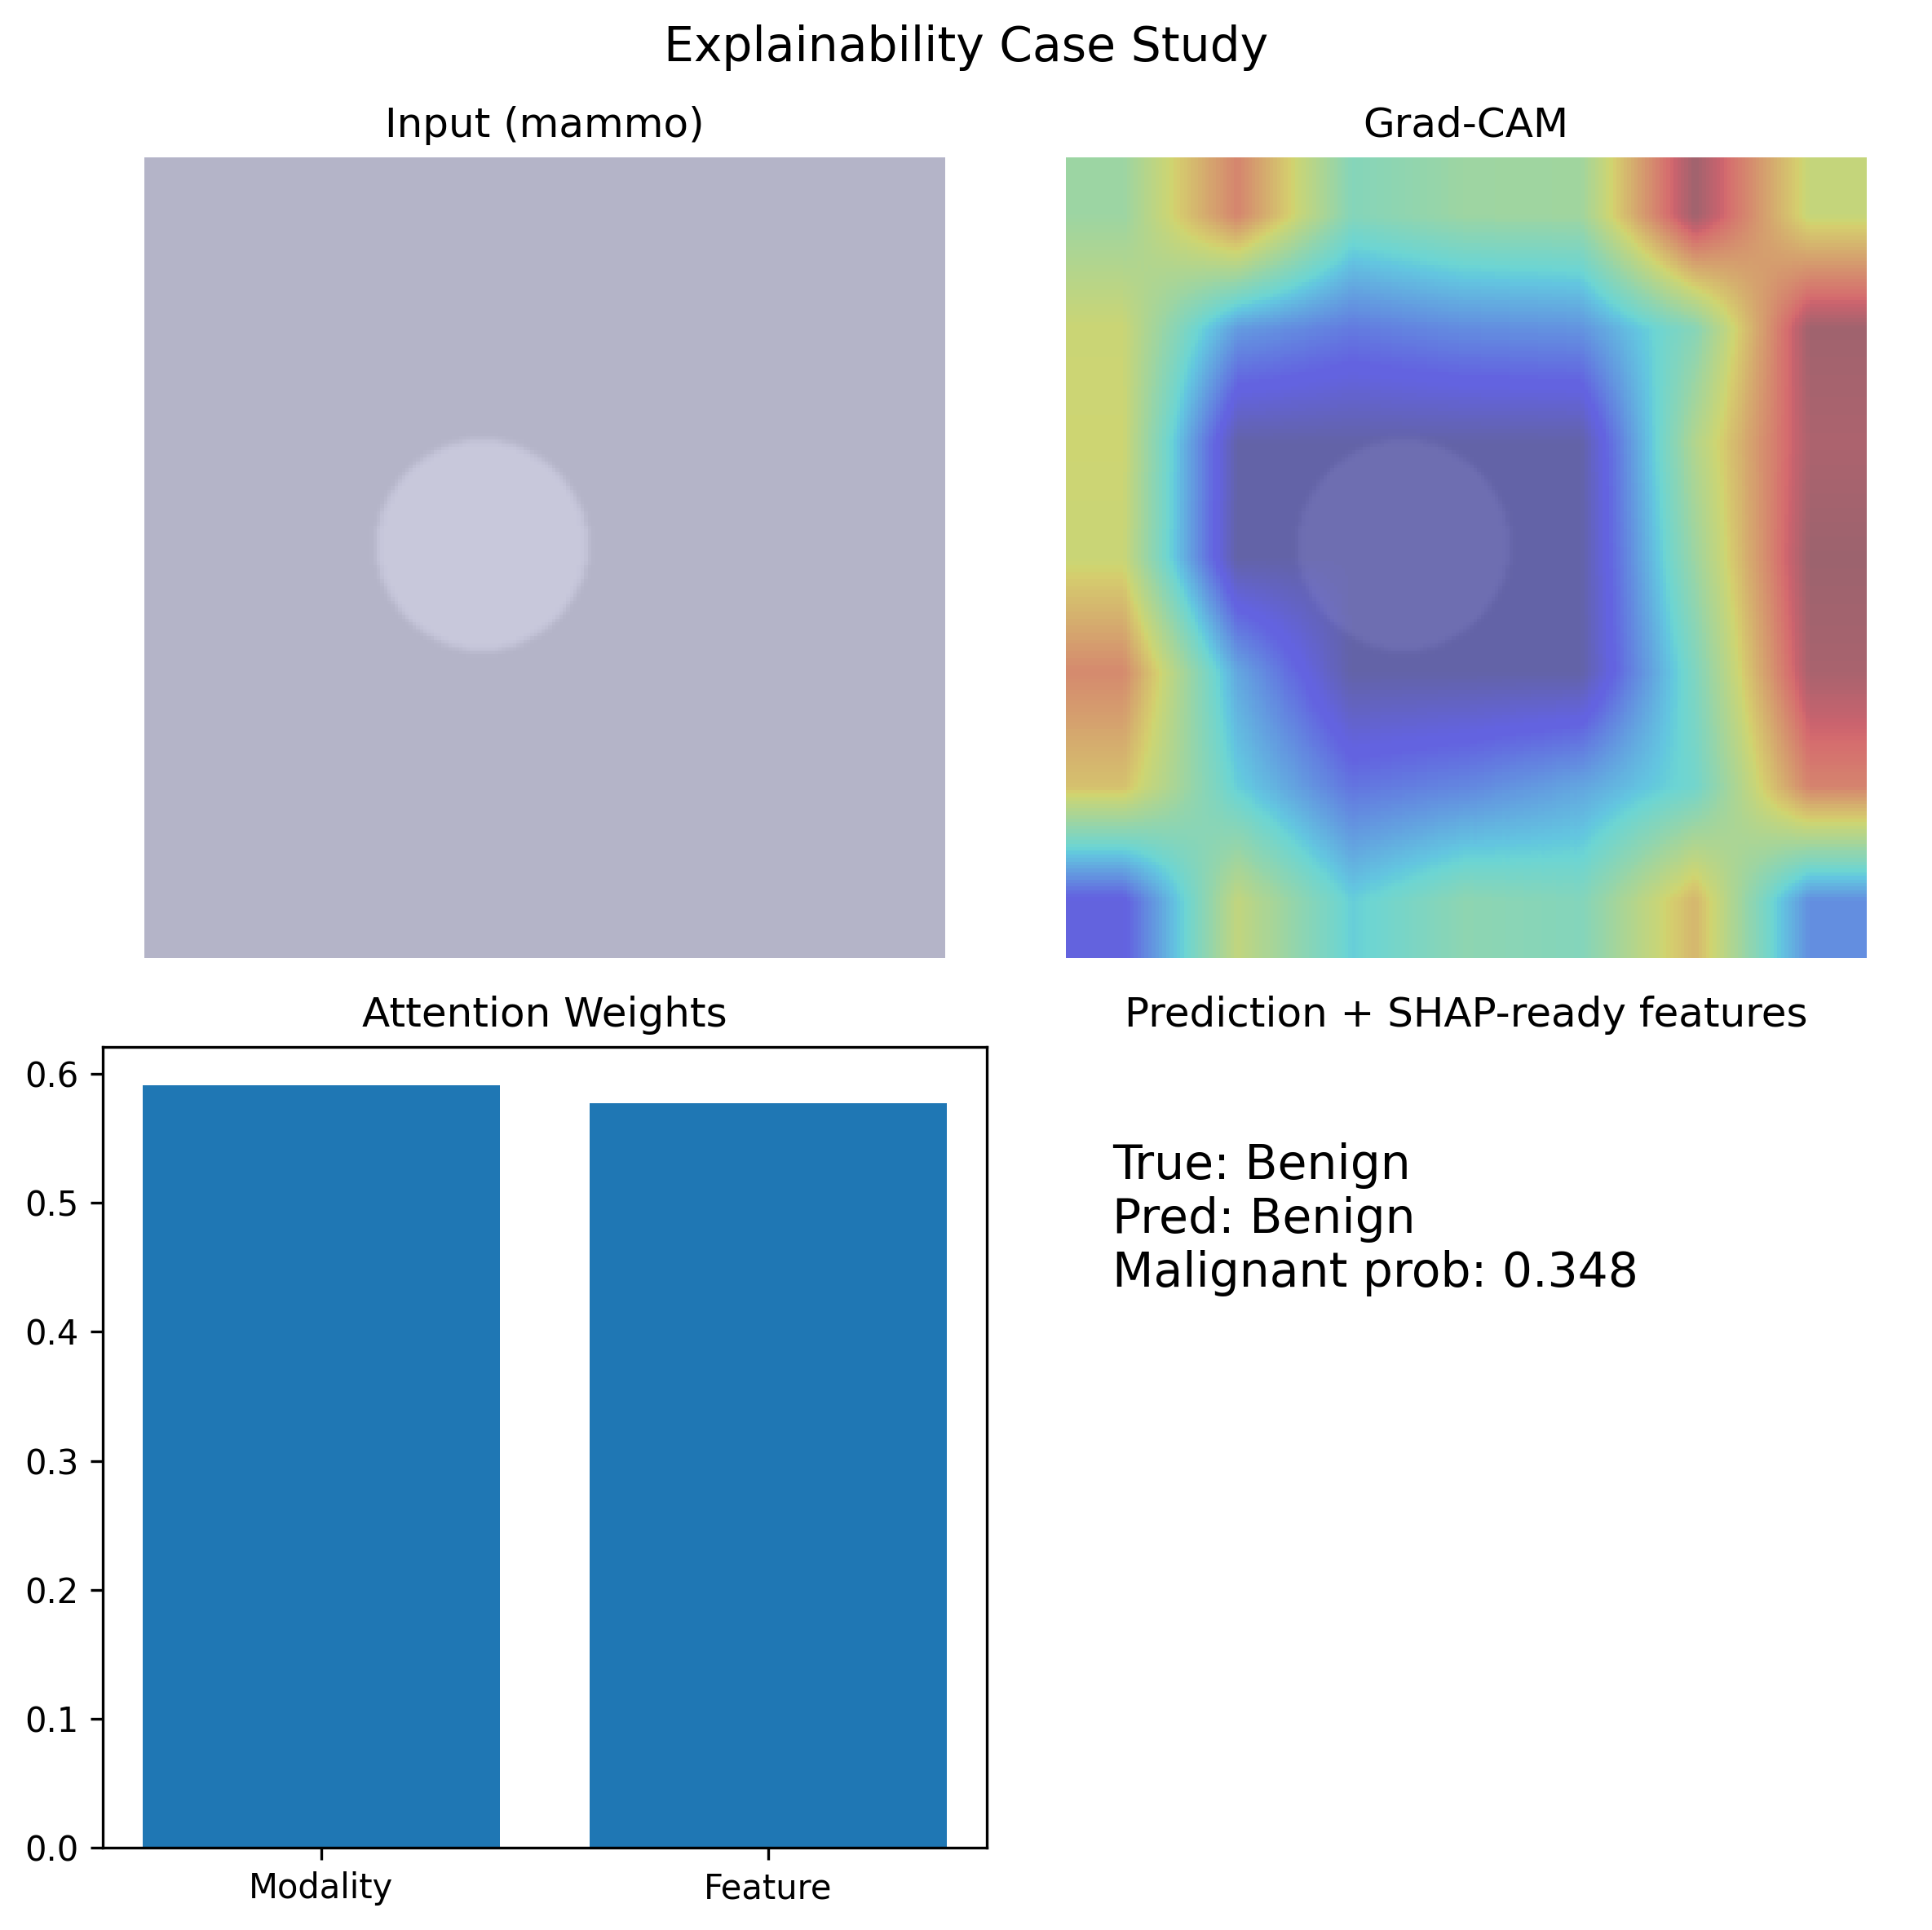
\includegraphics[width=\linewidth]{figures/case_study_0_mammo.png}
\caption{Explainability case study: input mammography image, Grad-CAM overlay, attention weights, and prediction summary.}
\label{fig:case}
\end{figure}

\section{Discussion}
The framework supports single-modality clinical workflows without paired data requirements. Quantum simulation results demonstrate feasibility; real hardware deployment remains future work. Thermography data scarcity may limit third-modality claims---mammography and ultrasound provide primary evidence.

\textbf{Limitations.} Simulation-only quantum evaluation; ultrasound and thermography experiments used synthetic placeholders pending BUSI download; two-stage training adds complexity. Histopathology-scale corpora ($\sim$200k patches) were not used---see \texttt{DATA\_SCALE.md}.

\section{Conclusion}
We presented a modality-level generalized hybrid quantum framework for breast cancer classification integrating Transformer-based invariance learning, VQC classification, and multi-method explainability. The approach enables scalable extension to MRI and histopathology modalities.

\section*{Code Availability}
Implementation, configs, and experiment scripts are available in the project repository.

\bibliographystyle{IEEEtran}
\bibliography{references}

\end{document}
